% ------------ begin cheatsheet
\documentclass[a4paper]{article}
\usepackage[a4paper,margin=0.05in]{geometry}
\usepackage{multicol}

\usepackage{amsmath, amssymb}
\usepackage[inline]{enumitem}
\usepackage{graphicx}

\usepackage{ulem}
\usepackage{makecell}

% horizontal list
\newlist{hlist}{enumerate*}{1}
\setlist[hlist]{label={}, afterlabel={}, itemjoin={{ \textbar{} }}}

% math
\newcommand{\abs}[1]{\left\lvert#1\right\rvert}

% envs
\newcommand{\oli}[1]{\begin{enumerate*}[label=(\arabic*)]#1\end{enumerate*}}

\graphicspath{ {./images/} }
\pagestyle{empty}
\setlength{\columnseprule}{0.3pt}

% reduce spacing before and after headers
\newcommand{\uppercaseandunderline}[1]{\uline{\uppercase{#1}}}

\makeatletter
\renewcommand{\section}{
  \@startsection{section}{1}{0pt}{1ex}{1.2ex} {\raggedleft\normalfont\large\bfseries\uppercaseandunderline}}
\renewcommand{\subsection}{
  \@startsection{subsection}{2}{0pt}{1ex}{1ex} {\raggedleft\normalfont\normalsize\bfseries\fbox}}
\renewcommand{\subsubsection}{
  \@startsection{subsubsection}{3}{0pt}{1ex}{0.8ex} {\raggedleft\normalfont\footnotesize\bfseries\uline}}
\renewcommand{\paragraph}{
  \@startsection{paragraph}{4}{0pt}{1.5ex}{-0.8em}{\normalfont\bfseries}}
% ------------ end cheatsheet

% ------------ begin code
\usepackage{xcolor}
\definecolor{dkgreen}{rgb}{0,0.6,0}
\definecolor{gray}{rgb}{0.5,0.5,0.5}
\definecolor{mauve}{rgb}{0.58,0,0.82}
\definecolor{lg}{rgb}{0.9,0.9,0.9}

% code environment
\usepackage{listings}
\lstset{
  %frame=tb, % adds top and bottom border
  aboveskip=1mm,
  belowskip=1mm,
  showstringspaces=false,
  columns=flexible,
  basicstyle={\footnotesize\ttfamily},
  numberstyle=\color{gray},
  keywordstyle=\color{blue}\textbf,
  commentstyle=\color{dkgreen},
  stringstyle=\color{mauve},
  breaklines=true,
  breakatwhitespace=true,
  backgroundcolor=\color{lg},
  tabsize=4
}
\newcommand{\ic}[1]{\lstinline{#1}}

% ------------ end code

\begin{document}
\footnotesize
\setlength{\abovedisplayskip}{0pt}
\setlength{\belowdisplayskip}{0pt}
\setlength{\abovedisplayshortskip}{0pt}
\setlength{\belowdisplayshortskip}{0pt}
\begin{multicols*}{3}
  \part*{\centering \underline{CS2104}}
\lstset{language=Haskell}
\section*{Haskell} \noindent
\begin{lstlisting}
error :: [Char] -> a
show :: Show a => a -> String
zip :: [a] -> [b] -> [(a, b)]

hoo :: (t1 -> t2 -> t2) -> t1 -> t2
hoo g x = g x (hoo g x)
\end{lstlisting}
\lstset{language=Prolog}
\section*{Prolog} \noindent
  An untyped (or dynamically-typed) language
  \subsection*{Atoms, Terms, Variables}
    \begin{itemize}[leftmargin=*]
      \item Atoms are constants. They must start with a lowercase letter
      \item Variables denote unknown values to be computed. They must start with a uppercase letter or underscore
      \item Terms are used to form tree-like data structures, e.g. \ic{cons(2,nil)}
      \item Can mix terms with variables, e.g. \ic{node(X,Y)}
    \end{itemize}
  \subsection*{Relations}
    \begin{lstlisting}
% Each predicate states a fact
% as a relation
father(john, mary).
male(john).
female(mary).

% Queries
?- father(X, mary).
X = john.
?- father(john, X), male(X).
false.
?- male(X); female(X).
X = john ;
X = mary.
    \end{lstlisting}
    \begin{itemize}[leftmargin=*]
      \item \ic{,} denotes conjunction (AND)
      \item \ic{;} denotes disjunction (OR)
    \end{itemize}
    \subsubsection*{Alternative for disjunction}
      \begin{lstlisting}
% Disjuncion implied
par(X,Y) :- father(X,Y).
par(X,Y) :- mother(X,Y).

% Equivalent:
par(X,Y) :- father(X,Y); mother(X,Y).
      \end{lstlisting}
    \subsubsection*{Number of solutions}
      \begin{itemize}[leftmargin=*]
        \item No solutions: \ic{false.} is shown immediately
        \item 1 solution: solution is shown immediately with full stop.
        \item Multiple solutions: one solution is shown
          \begin{itemize}[leftmargin=*]
            \item Typing \ic{.} stops displaying other possible solns
            \item Typing \ic{;} goes to the next soln
          \end{itemize}
      \end{itemize}
  \subsection*{Horn clauses}
    \begin{lstlisting}
% Horn clause
res(X) :- father(john, X), female(X).
?- res(X).
X = mary.
    \end{lstlisting}
    \begin{itemize}[leftmargin=*]
      \item Can store logical formula into a single predicate
    \end{itemize}
    \begin{lstlisting}
% Good
ancestor(X,Y) :- parent(X,Y).
ancestor(X,Y) :- parent(X,Z), ancestor(Z,Y).

% Bad (infinite loop)
ancestor(X,Y) :- parent(X,Y).
ancestor(X,Y) :- ancestor(Z,Y), parent(X,Z).
    \end{lstlisting}
    \begin{itemize}[leftmargin=*]
      \item Can be recursive, but left recursion may result in infinite loop
    \end{itemize}
  \subsection*{Unification}
    \begin{itemize}[leftmargin=*]
      \item Mechanism that Prolog uses to match two terms
      \item Unification \ic{t1=t2} may contain variables. The system tries to compute a substitution for the variables to make the two terms equal
      \item Once a variable is bound, it cannot be changed
    \end{itemize}
    \begin{lstlisting}
a=X              % X=a
a=b              % fail, unique atoms
                 % are diff
n(a,X) = n(Y,b)  % X=b, Y=a
n(a,X) = n(X,b)  % fail, X cannot be
                 % both a and b
n(a,X) = n(X,a)  % X=a
    \end{lstlisting}
    \subsubsection*{Algorithm}
      \begin{enumerate}[leftmargin=*]
        \item Given initial unification request $\Sigma_i = \Pi_1, \Sigma_2 = \Pi_2, \cdots$
        \item If $\Sigma_1$ or $\Pi_1$ is a variable, add $\Sigma_1 = \Pi_1$ to the answer, and apply it as substitution to the remaining list of unifications. Go to last step
        \item If the predicate name for $\Sigma_1$ and $\Pi_1$ are different, exit with failure.
        \item If the number of parameters for $\Sigma_1$ and $\Pi_1$ are different, exit with failure.
        \item Denote by $\Sigma_{11}, \Sigma_{12}, \cdots, \Sigma_{1k}$ the arguments of $\Sigma_1$, and similarly $\Pi_{11}, \Pi_{12}, \cdots, \Pi_{1k}$ the arguments of $\Pi_1$.
        \item Set unification request to
          \begin{gather*}
            \Sigma_{11} = \Pi_{11}, \Sigma_{12} = \Pi_{12}, \cdots, \Sigma_{1k}
            = \Pi_{1k}, \\
            \Sigma_2 = \Pi_2, \cdots
          \end{gather*}
        \item If unification request is not empty, go to first step. Otherwise, terminate with success
      \end{enumerate}
  \subsection*{Resolution}
    \begin{itemize}[leftmargin=*]
      \item Process of answering a query
    \end{itemize}
    \subsubsection*{Algorithm}
      \begin{itemize}[leftmargin=*]
        \item Given query \ic{A1, A2, ... An}
        \item Pick a matching rule from the program and rename its variables: \ic{H :- B1, B2, ... Bk}
        \item New goal: \ic{(H=A1), B1,B2,...,Bk, A2,...An}
        \item Variable bindings may be generated by the unification request \ic{H=A1}. Add them to the answer, replacing bound variables by its substitution over the entire query
        \item Go back to step 1 if query is not empty. Else, return the answer
      \end{itemize}
    \subsubsection*{Resolution tree example}
      \begin{center}
        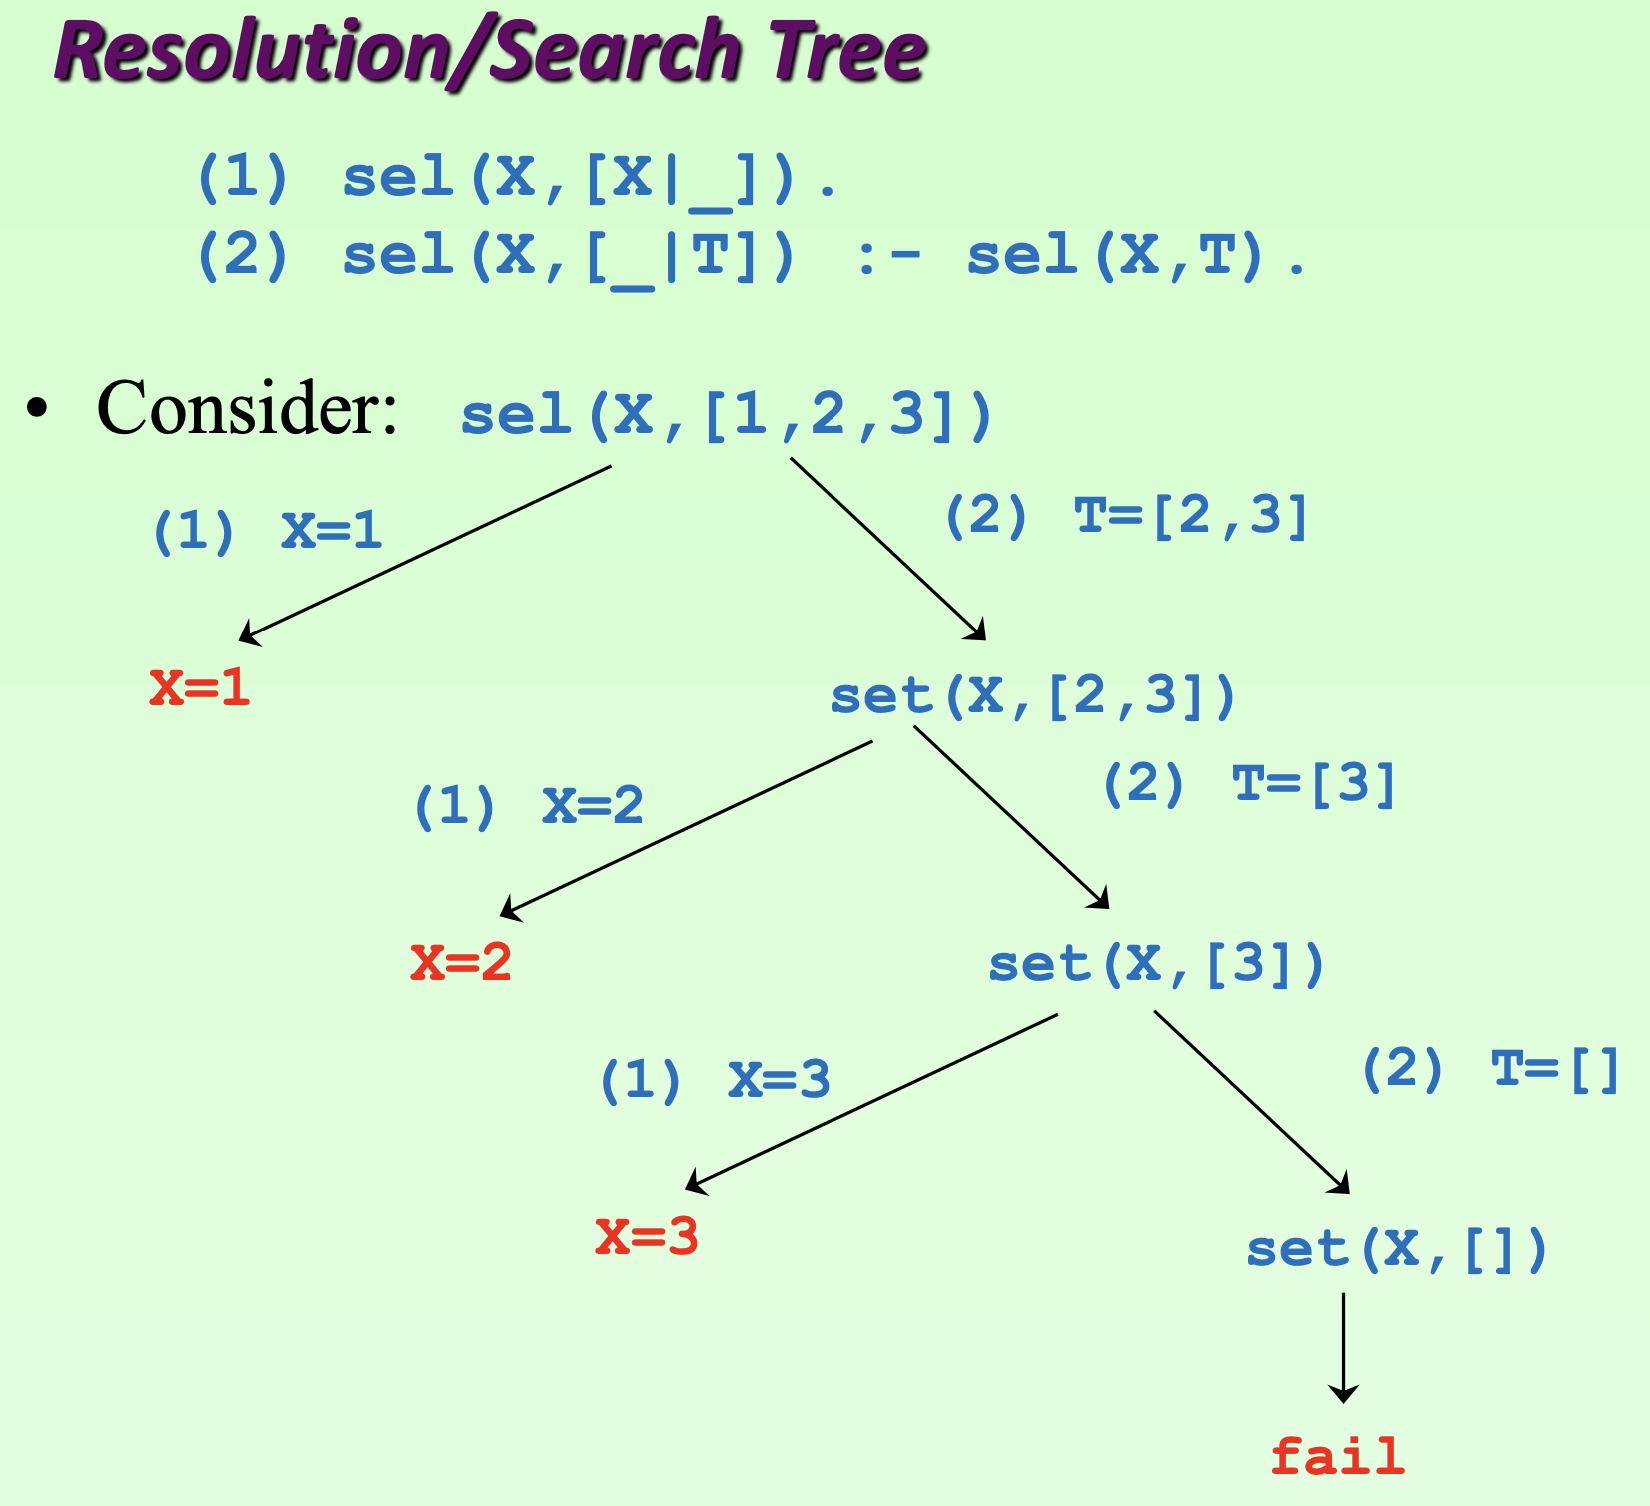
\includegraphics[width=\columnwidth]{L8/resolution_tree}
      \end{center}
  \subsection*{Lists} \noindent
    Denoted by square brackets with elements separated by comma: \ic{[mary, [], n(A), [1,2,3], X]}
    \subsubsection*{Append}
      \begin{lstlisting}
% Params may be input/output
append([],Y,Y).
append([X|Xs],Y,[X|Rs]) :- append(Xs,Y,Rs).

% Join lists, Z as output
?- append([1,2],[3],Z).
Z = [1,2,3].

% Compute difference, Y as output
?- append([1,2],Y,[1,2,3]).
Y = [3].

% Split list
?- append(X,Y,[1,2]).
X=[], Y=[1,2];
X=[1], Y=[2];
X=[1,2], Y=[];

% Prefix a list
?- append(X,_,[1,2]). 
X=[]; X=[1]; X=[1,2]; X=[1,2,3];
      \end{lstlisting}
      \begin{itemize}[leftmargin=*]
        \item Can represent the backtracking performed by resolution using a search tree
        \item One outgoing edge per predicate clause
        \item Answers are found at child nodes. All answers are provided using \ic{;} (OR) to represent multiple possibilities
      \end{itemize}
  \subsection*{Reverse}
    \begin{lstlisting}
rev([],[]).
rev([X|Xs],Y):- rev(Xs,Y2),append(Y2,[X],Y).
?- rev([1,2,3],Y).
Y = [3,2,1].
?- rev(X,[1,2,3]).
X = [3,2,1].
    \end{lstlisting}
    \begin{itemize}[leftmargin=*]
      \item Note: this implementation of reverse results in unterminated search after finding the first (only reasonable) answer.
    \end{itemize}
    \begin{lstlisting}
?- rev(X,X).
X = [] ;
X = [_] ;
X = [_A, _A] ;
X = [_A, _, _A] ;
...
    \end{lstlisting}
  \subsection*{Select (list membership)}
    \begin{lstlisting}
sel(X,[X|_]).
sel(X,[_|T]) :- sel(X,T).

% Fails immediately since both clauses
% are not applicable
?- sel(X,[]).
false.

?- sel(3,[1,3,5]).
true.
?- sel(X,[1,3,5]).
X=1; X=3; X=5.
    \end{lstlisting}
  \subsection*{Arithmetic}
    \subsubsection*{is-Operator}
      \begin{lstlisting}
X is 3+4     % X=7
7 is 3+4     % succeed
7 is X+4     % fail, RHS must be
             % fully instantiated
      \end{lstlisting}
    \subsubsection*{Comparison}
      \begin{itemize}[leftmargin=*]
        \item Relations \ic{>, <, >=, =<, =\=, =:=} compares two arithmetic expressions that must be fully instantiated
        \item Operator \ic{=} is for term unification
      \end{itemize}
    \subsubsection*{Factorial}
      \begin{lstlisting}
fact(0,1).
fact(N,R) :- N>0, M is N-1, fact(M, R1), R is N*R1.

?- fact(5,R).
R = 120.
?- fact(X,120).
% ERROR: >/2: Arguments are not sufficiently
% instantiated. Matches with second clause,
% then N>0 cannot be evaluated.
      \end{lstlisting}
  \subsection*{Negation}
    \begin{itemize}[leftmargin=*]
      \item Prolog is based on closed world assumption. Instantiation of predicates are true. If the instantiation does not exist, then it is assumed to be false.
    \end{itemize}
    \begin{lstlisting}
father(john,mary).

?- father(john,kerry).
false.
    \end{lstlisting}
    \begin{itemize}[leftmargin=*]
      \item If we have the clause \ic{male(X) :- not(female(X)).}, then need only specify facts on female
      \item Above clause says if a person cannot be proven to be female, then assume the person is male
    \end{itemize}
  \subsection*{Cut}
    \begin{itemize}[leftmargin=*]
      \item Cut operator \ic{!}
      \item Used to stop backtracking
    \end{itemize}
    \begin{lstlisting}
teach(dr_X, compsci).
teach(dr_X, math).
teach(dr_X, physics).
teach(dr_Y, chemistry).
study(alice, chemistry).
study(bob, math).
study(charlie, physics).

% All students taught by dr_X
?- teach(dr_X, Subj), study(Stud, Subj).
Subj = math, Stud = bob;
Subj = physics, Stud = charlie;

% teach first matches on compsci
% cut prevents further backtracking
?- teach(dr_X, Subj), !, study(Stud, Subj).
false.
    \end{lstlisting}
  \subsection*{Impure Prolog}
    \begin{itemize}[leftmargin=*]
      \item \ic{atom(X), var(X), integer(X)}
      \item \ic{write(X)} outputs the binding of X
    \end{itemize}
  \subsection*{Constraint Solving}
    \begin{itemize}[leftmargin=*]
      \item \ic{use_module(library(clpfd)).}
      \item Regular prolog comparison (e.g. \ic{A > B}) requires both A and B to be instantiated to evaluate
      \item Constraint solving uses \ic{A #> B}, obtaining \\
        \ic{B #=< A + -1}
    \end{itemize}
    \begin{lstlisting}
?- X #> 3.
X in 4..sup.
?- X #\= 10.
X in inf..9\/11..sup.
?- 3*X #= 9.
X=3.
?- X*X #= 9.
X=3\/-3.
    \end{lstlisting}
    \subsubsection*{Factorial}
      \begin{itemize}[leftmargin=*]
        \item Constraint solving allows both params as input
      \end{itemize}
      \begin{lstlisting}
cfact(0,1).
cfact(N,R) :- N #> 0, M #= N-1, 
      R #= N*R1, cfact(M, R1).
?- cfact(5,R).
R=120.
?- cfact(N,120).
N=5.
      \end{lstlisting}
    \subsubsection*{Puzzle Solving}
      \begin{lstlisting}
:- use_module(library(clpfd)).

puzzle([S,E,N,D]+[M,O,R,E]=[M,O,N,E,Y]) :-
  Vars = [S,E,N,D,M,O,R,Y],
  Vars ins 0..9,
  all_different(Vars),
            S*1000 + E*100 + N*10 + D +
            M*1000 + O*100 + R*10 + E #=
  M*10000 + O*1000 + N*100 + E*10 + Y,
  M #\= 0, S #\= 0.

?- puzzle(As+Bs=Cs),label(As).
As = [9, 5, 6, 7],
Bs = [1, 0, 8, 5],
Cs = [1, 0, 6, 5, 2];
      \end{lstlisting}
      \begin{itemize}[leftmargin=*]
        \item Without label, we have a partially solved answer
        \item Label tells the CLP to find solutions for the given variables
      \end{itemize}
\lstset{language=Scala}
\section*{Scala}
  \subsection*{Misc}
    \subsubsection*{Pure vs imperative}
      \begin{itemize}[leftmargin=*]
        \item Pure functions are:
          \begin{hlist}
            \item Easier to reason/debug
            \item Less error prone
            \item Easily composable
          \end{hlist}
        \item Imperative features are still needed
        \item Use pure functions where possible, and imperative features where necessary
      \end{itemize}
    \subsubsection*{Mutable class}
      \begin{lstlisting}
class Point(xc: Int, yc: Int) extends .. {
  var x: Int = xc
  var y: Int = yc
  def move(dx: Int, dy: Int) {
    x = x + dx
    y = y + dy
  }
  override def toString(): String
    = "(" + x + ", " + y + ")";
}
      \end{lstlisting}
    \subsubsection*{Modifiers}
      \begin{itemize}[leftmargin=*]
        \item \ic{val} for constant. Allows getter
        \item \ic{var} for mutability. Allows getter, setter
        \item \ic{private} disallows getter, setter
        \item \ic{protected} allows access only via base and sub-classes
      \end{itemize}
    \subsubsection*{Mutable reference}
      \begin{itemize}[leftmargin=*]
        \item Essence of mutation can be captured by a polymorphic \ic{Ref} class with mutation:
      \end{itemize}
      \begin{lstlisting}
class Ref[A](v:A):
  var vl = v
  def get: A =
    vl
  def update(nv:A): Unit =
    vl = nv
end Ref
      \end{lstlisting}
  \subsection*{Loops}
    \subsubsection*{For loop}
      \begin{lstlisting}
// Prints 0 to 3 (inclusive)
for (i <- 0 to 3)
  println(s"i = $i")
// Prints 3 to 0 (inclusive)
for (i <- 3 to 0 by -1)
  println(s"i = $i")
// Prints 3 to 0 (inclusive)
for (i <- (0 to 3).reverse)
  println(s"i = $i")
      \end{lstlisting}
    \subsubsection*{While loop}
      \begin{lstlisting}
// Prints 3 to 0 (inclusive)
var i = 3
while (i >= 0) {
  println(s"i = $i")
  i = i-1
}
      \end{lstlisting}
  \subsection*{Sequence comprehension}
    \begin{lstlisting}
// Vector((1,2), (1,3), (2,3))
val f_lst =
  for (i <- 1 to 3; j <- 1 to 3 if i<j)
    yield (i,j)
    \end{lstlisting}
  \subsection*{List iterator}
    \begin{lstlisting}
for (name <- lst) {
  ..code..
}
lst.forEach((name: String) => ..code..)
    \end{lstlisting}
  \subsection*{Hash table/map}
    \begin{itemize}[leftmargin=*]
      \item Implements generic dictionary
    \end{itemize}
    \begin{lstlisting}
class HashMap[K, V] extends AbstractMap[K, V]
// Initialization with expected load factor
new HashMap(initialCapacity: Int, loadFactor: Double)
// Operations
tbl.+=(k,v)   // to add (k,v) to tbl
tbl.get(k)    // return binding of k
tbl.remove(k) // remove binding of k
    \end{lstlisting}
    \begin{itemize}[leftmargin=*]
      \item Can be used for memoization
      \item If hash map is localized in the function, then when viewed from outside it appears as a pure function
    \end{itemize}
    \begin{lstlisting}
// fib with memoization
def fib_memo(n: Int): Int = {
  val tbl = new HashMap[Int, Int]()
  def aux(n: Int): Int = {
    if (n <= 1) 1
    else {
      val r = tbl.get(n)
      r match {
        case None => {
          val ans = aux(n-1) + aux(n-2)
          tbl.+=((n, ans))
          ans
        }
        case Some(ans) => ans
      }
    }
  }
  aux(n)
}
    \end{lstlisting}
\section*{Scala OOP} \noindent
  \subsection*{OOP Principles}
    \begin{itemize}[leftmargin=*]
      \item \textbf{Abstraction} allows implementation details to be hidden via private fields and methods
      \item \textbf{Encapsulation} binds data fields and methods together
      \item \textbf{Inheritance} is facilitated by sub-class mechanism with inherited fields and methods
      \item \textbf{Polymorphism} is supported by type variables and class hierarchy
    \end{itemize}
  \subsection*{Scala vs Java}
    \begin{itemize}[leftmargin=*]
      \item No static fields/methods. Workaround: use a singleton class with keyword \ic{object} instead of \ic{class}
      \item No primitive types
    \end{itemize}
  \subsection*{Class hierarchy}
    \begin{center}
      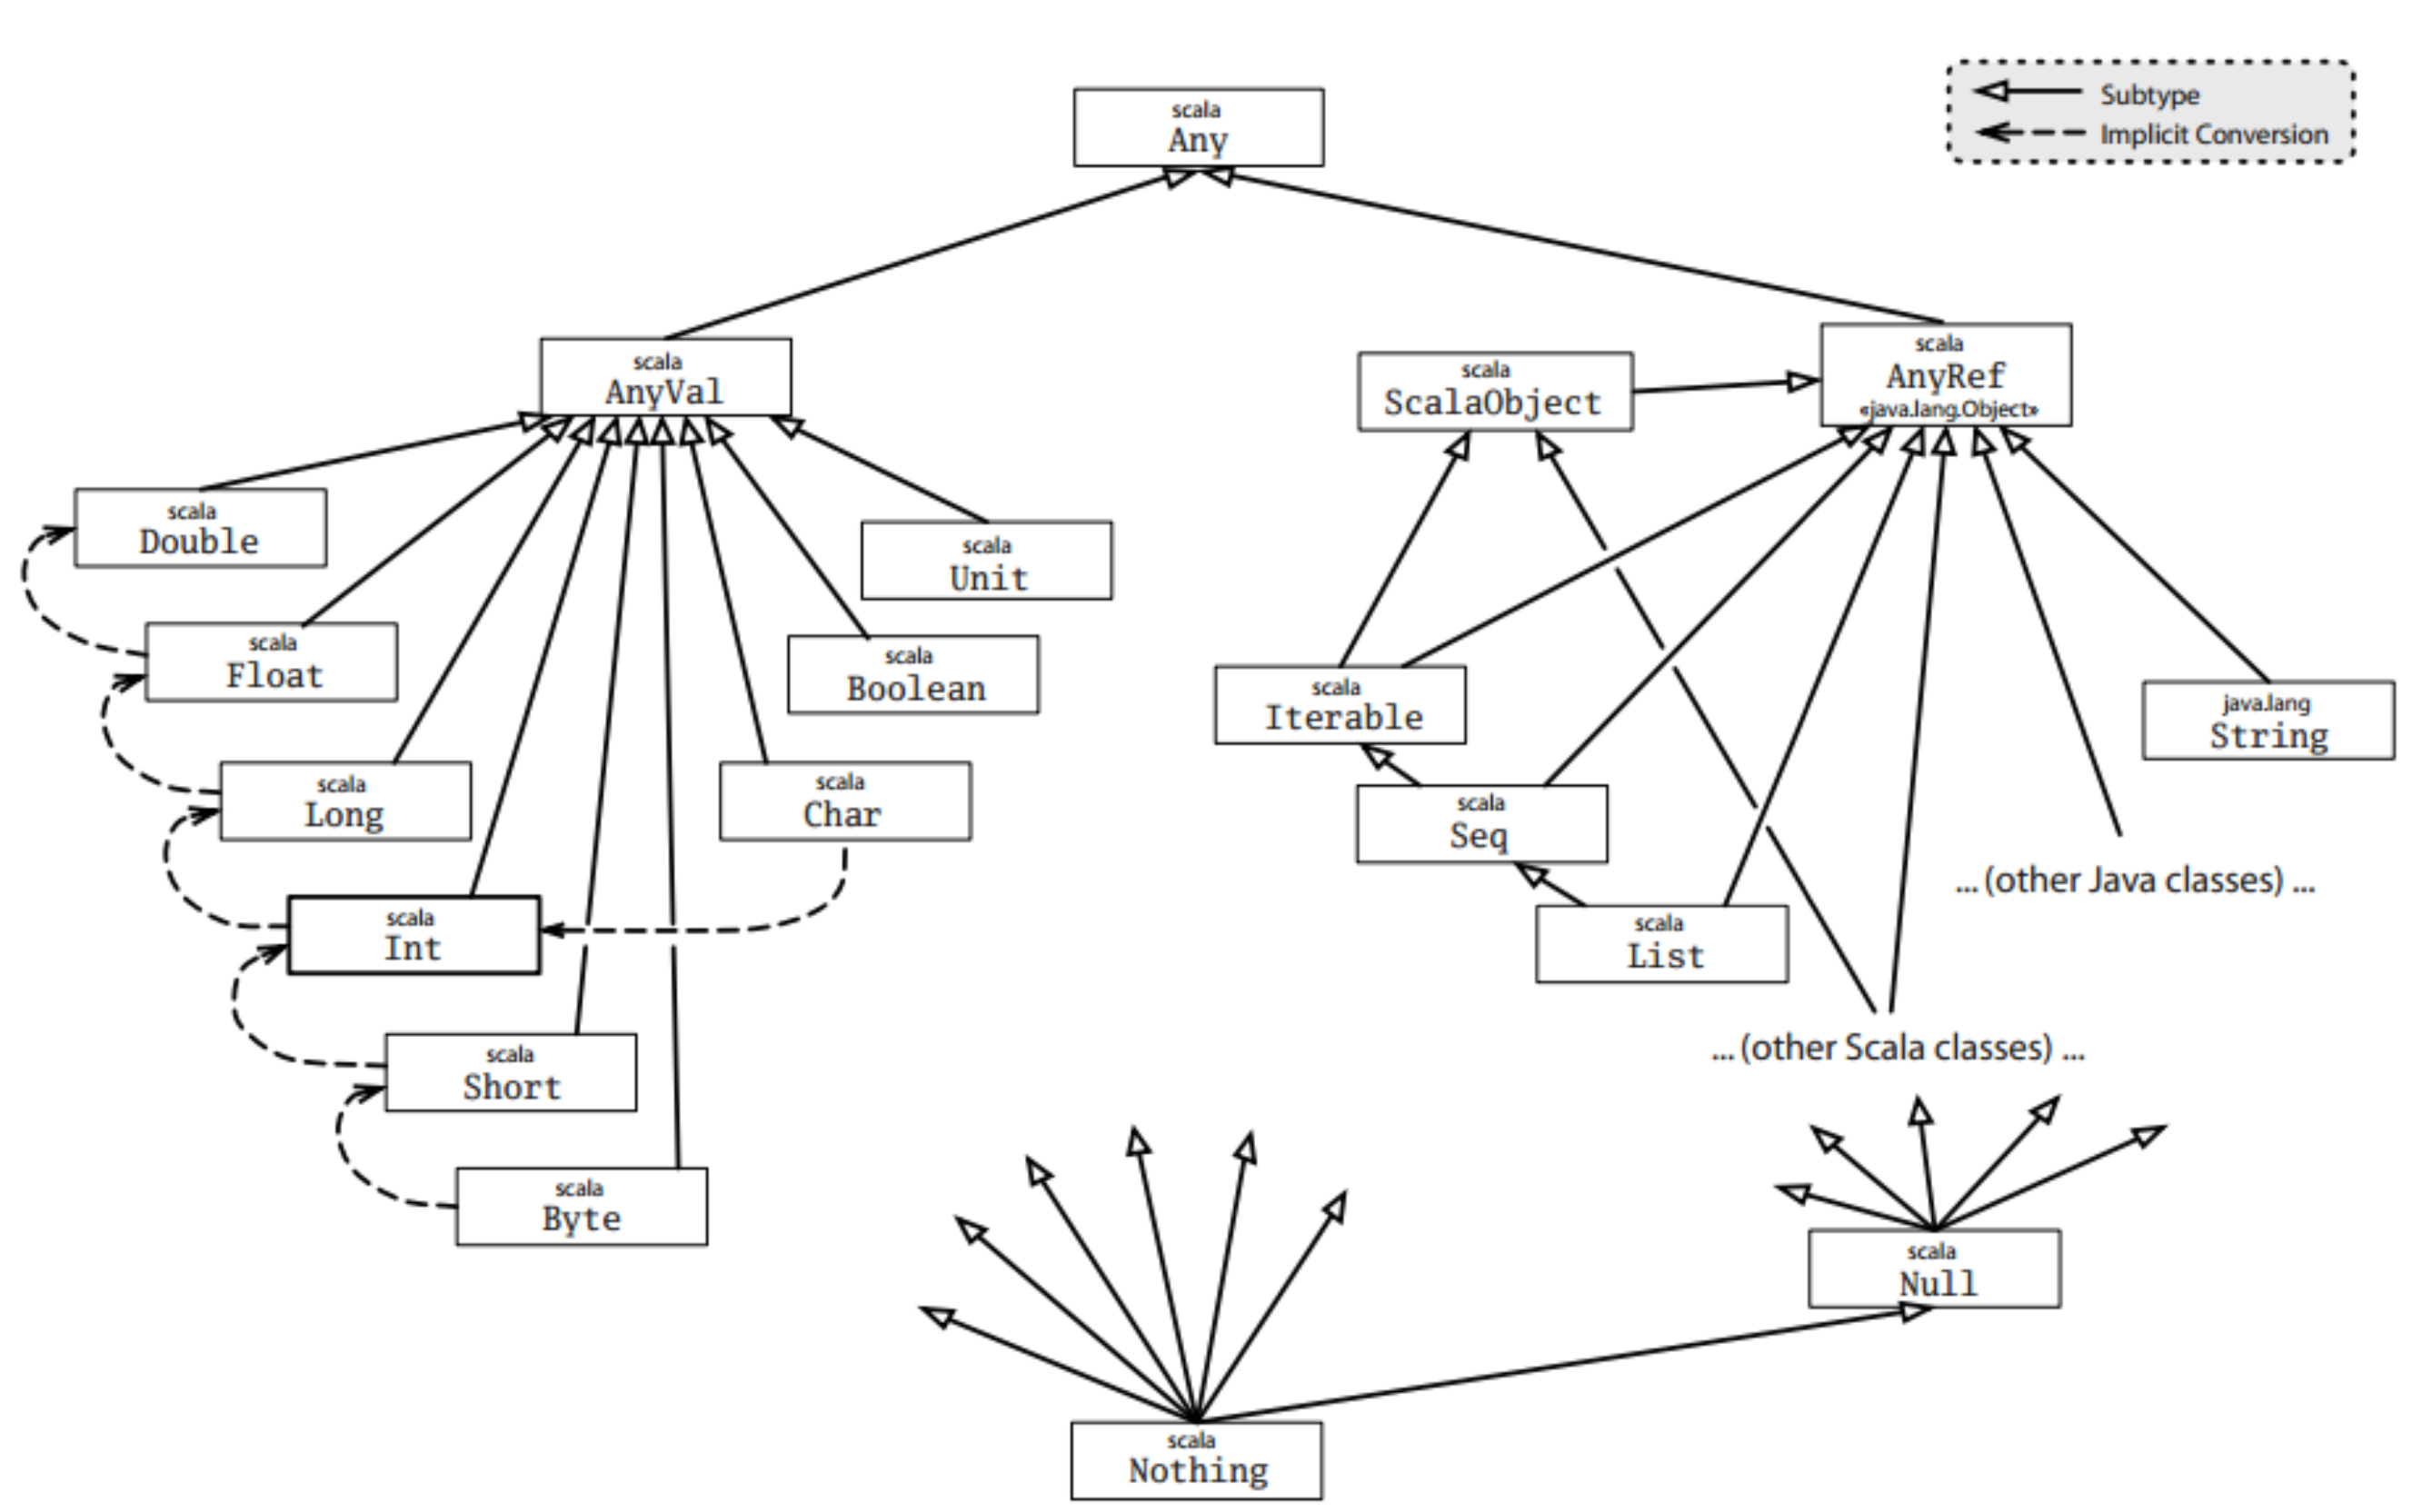
\includegraphics[width=\columnwidth]{L10/class_hierarchy}
    \end{center}
    \begin{itemize}[leftmargin=*]
      \item Every user class
        \begin{itemize}[leftmargin=*]
          \item is indirectly a subclass of \ic{scala.AnyRef}
          \item implicitly extends trait \ic{scala.ScalaObject}
        \end{itemize}
    \end{itemize}
    \subsubsection*{Product types} \noindent
      Includes tuples and records; Similar to conjunction $a \land b$
      \begin{lstlisting}
class Pair[A,B] = (a, b)
      \end{lstlisting}
    \subsubsection*{Sum types} \noindent
      Includes ordinals and general algebraic data types; Similar to disjunction $a \lor b$
      \begin{lstlisting}
abstract class Either[A,B]
case class Left[A] extend Either[A,B]
case class Right[B] extend Either[A,B]
      \end{lstlisting}
  \subsection*{Type inference}
    \begin{itemize}[leftmargin=*]
      \item Types can either be declared or inferred
      \item Can infer type of
        \begin{itemize}[leftmargin=*]
          \item variable (through its initialization)
          \item results of non-recursive method
          \item type instantiation of polymorphic methods
        \end{itemize}
      \item May fail
    \end{itemize}
    \begin{lstlisting}
class MyPair[A, B](x: A, y: B);
object InferenceTest3 extends Application {
  def id[T](x: T) = x
  // type: MyPair[Int, String]
  val p = new MyPair(1, "scala")
  val q = id(1) // type: Int
}

// Explicit instantiation
val x: MyPair[Int, String] = new MyPair[Int, String](1, "scala")
val y: Int = id[Int](1)

// Failure
// Compilation error: Overloaded or recursive method fac needs return type
object Test {
  def fac(n: Int) = if (n == 0) 1 else n * fac(n - 1)
}
    \end{lstlisting}
    \subsubsection*{Runtime type representation}
      \begin{itemize}[leftmargin=*]
        \item Use \ic{classOf[T]} to get string representation of a type
        \item Use \ic{var.getClass()} to get the representation of runtime type for object
      \end{itemize}
  \subsection*{Abstract classes}
    \begin{itemize}[leftmargin=*]
      \item Provides a common definition of a base class that multiple derived classes can share
      \item Supports generic classes
      \item Can have deferred/abstract type, deferred value definition
    \end{itemize}
    \begin{lstlisting}
abstract class Buffer[T] {
  val element: T
}
abstract class SeqBuffer[U,T<:Seq[U]] extends Buffer[T] {
  def length = element.length
}
    \end{lstlisting}
  \subsection*{Traits}
    \begin{itemize}[leftmargin=*]
      \item Can have fields, methods
      \item May have default impl for some methods
      \item Do not have constructor parameters
      \item Can be extended by other traits, abstract classes, concrete classes, and case classes
      \item More expressive than Java interfaces
    \end{itemize}
    \begin{lstlisting}
// Similar to Eq type class in Haskell
trait Similarity {
  def isSimilar(x: Any): Boolean
  def isNotSimilar(x: Any): Boolean = !isSimilar(x)
}
    \end{lstlisting}
  \subsection*{Mixins}
    \begin{itemize}[leftmargin=*]
      \item Classes can only have one superclass, but have many mixins
      \item Use mixins to derive from multiple classes
    \end{itemize}
    \begin{lstlisting}
abstract class AbsIterator {
  type T
  def hasNext: Boolean
  def next: T
}
// A mixin
trait RichIterator extends AbsIterator {
  def foreach(f: T => Unit)
    { while (hasNext) f(next) }
}
// A concrete class
class StringIterator(s: String) extends AbsIterator {
  type T = Char
  private var i = 0
  def hasNext = i < s.length()
  def next = { val ch = s charAt i; i += 1; ch }
}
// A mixin class composition
object StringIteratorTest {
  def main(args: Array[String]) {
  class Iter extends StringIterator(args(0)) with RichIterator
    val iter = new Iter
    iter foreach println
  }
}
    \end{lstlisting}
  \subsection*{Polymorphism}
    \subsubsection*{Method polymorphism}
      \begin{itemize}[leftmargin=*]
        \item Same method name takes different forms
        \item \textbf{Static polymorphism}: Overloading
        \item \textbf{Dynamic polymorphism}: Overriding
      \end{itemize}
    \subsubsection*{Type polymorphism}
      \begin{itemize}[leftmargin=*]
        \item \textbf{Parametric polymorphism}: Function can take different types
        \item \textbf{Sub-class polymorphism}: A list with type \ic{List[A]} contains elems that are sub-classes of \ic{A}
        \item Note: Scala 2 \ic{val} cannot be polymorphic, but Scala 3 \ic{val} can
      \end{itemize}
    \subsubsection*{Abstract type definition}
      \begin{lstlisting}
// Java vs Scala
? extends T = +T
? super T = -T
T = T
? = _
      \end{lstlisting}
  \subsection*{Variances}
    \begin{itemize}[leftmargin=*]
      \item \ic{<:} is read ``is a subtype of''
      \item Subclass $\implies$ subtype
        \[ \frac{T1 \text{ is subclass of } T2}{T1 <: T2} \]
      \item Covariance subtyping for read-only (OUT) structures, e.g. \ic{List[Int] <:} \ic{List[Object]}
        \[ \frac{T2 <: T4}{List[+T2] <: List[+T4]} \]
      \item Invariance subtyping for mutable (IN/OUT) structures, e.g. \ic{Array[Int] <:} \ic{Array[Int]}
        \[ \frac{T2 = T4}{Array[T2] = Array[T4]} \]
      \item Contravariance subtyping for write-only (IN) structures, e.g. \ic{Printer[Object] <:} \ic{Printer[Int]}
        \[ \frac{T2 <: T4}{Printer[-T4] <: Printer[-T2]} \]
      \item Function subtyping
        \[ \frac{I2<:I1 \qquad\qquad O1 <: O2}{Func[-I1,+O1] <: Func[-I2,+O2]} \]
    \end{itemize}
  \subsection*{Packages}
    \begin{itemize}[leftmargin=*]
      \item Defines a set of member classes, objects, and packages
      \item Private: visible only for other members of the package
      \item Protected: accessible from all code inside the package
    \end{itemize}
  \subsection*{Imports}
    \begin{itemize}[leftmargin=*]
      \item Implicit imports: packages \ic{java.lang}, \ic{scala}, the object \ic{scala.Predef}
    \end{itemize}
    \begin{lstlisting}
// all members of p
// (analogous to import p.* in Java).
import p._
// the member x of p.
import p.x
// the member x of p renamed as a.
import p.{x => a}
// the members x and y of p.
import p.{x, y}
// the member z of p2, itself member of p1.
import p1.p2.z
    \end{lstlisting}
\section*{Scala FP}
  \begin{itemize}[leftmargin=*]
    \item Every function is an object
    \item Functions are first-class values. Can be
      \begin{itemize}[leftmargin=*]
        \item Passed as argument
        \item Returned as result
        \item Stored in data structures
      \end{itemize}
    \item Anonymous functions allowed
  \end{itemize}
  \begin{lstlisting}
object XXX extends App {
  def inc (x:int) : int = x+1
}
// Anonymous functions
(x:Int) => x+1
new Function1[Int, Int] {
  def apply(x: Int): Int = x + 1
}
  \end{lstlisting}
  \subsection*{Handling errors}
    \subsubsection*{Option type}
      \begin{lstlisting}
enum Option[+T]:
  case None
  case Some(x:T)

def divide(x:Float,y:Float): Option[Float] {
  if (y==0) None
  else Some(x/y)
}
      \end{lstlisting}
    \subsubsection*{Either type}
      \begin{lstlisting}
enum Either[+T,+S]:
  case Left(x:T)
  case Right(x:S)

def divide(x:Float,y:Float): Either[String,Float] {
  if (y==0) Left("cannot div by 0")
  else Right (x/y)
}
      \end{lstlisting}
    \subsubsection*{Exception handling}
      \begin{itemize}[leftmargin=*]
        \item Not referentially transparent
      \end{itemize}
      \begin{lstlisting}
class DivideByZero extends RuntimeException

def divide(x:Float,y:Float):Float {
  if (y==0) throw new DivideByZero
  else (x/y)
}
      \end{lstlisting}
  \subsection*{Case classes}
    \begin{itemize}[leftmargin=*]
      \item Allow constructor parameters to be used in pattern-matching
      \item \ic{new} keyword not required
    \end{itemize}
    \begin{lstlisting}
// Untyped lambda calculus
abstract class Term
  case class Var(name: String) extends Term
  case class Fun(arg: String, body: Term) extends Term
  case class App(f: Term, v: Term) extends Term

val x = Var("x")
Console.println(x.name)
    \end{lstlisting}
  \subsection*{Pattern matching}
    \begin{itemize}[leftmargin=*]
      \item First-match policy
      \item \ic{match} keyword allows pattern matching function to be applied to an object
      \item Can match against different types
      \item \ic{_} indicates the default catch all
    \end{itemize}
    \begin{lstlisting}
object MatchTest1 extends Application {
  def matchTest(x: Int): String = x match {
    case 1 => "one"
    case 2 => "two"
    case _ => "many"
  }
  println(matchTest(3))
}
    \end{lstlisting}
  \subsection*{Lists}
    \begin{lstlisting}
val fruit = List("apple", "orange", "pear")
val f2="apple" :: "orange" :: "pear" :: Nil

fruit.head // apple
fruit.tail // List(orange, pear)
fruit.isEmpty // false

val List(a,b,c) = fruit
a: String = apple
b: String = orange
c: String = pear

val a :: b :: rest = fruit
a: String = apple
b: String = orange
rest: List[String] = List(pear)
    \end{lstlisting}
    \subsubsection*{List operations}
      \begin{lstlisting}
def length[T](xs:List[T]):Int =
  xs match {
    case List() => 0
    case x :: xs1 => 1+length(xs1)
  }
def append[T](xs: List[T], ys: List[T]): List[T] =
  xs match {
    case List()   => ys
    case x :: xs1 => xs :: append(xs1, ys)
  }
def sum(xs: List[Int]): Int = (0 /: xs) (_ + _)
def prod(xs: List[Int]): Int = (1 /: xs) (_ * _)
      \end{lstlisting}
  \subsection*{Higher-order functions}
    \begin{itemize}[leftmargin=*]
      \item Functions can be used as parameters, results, inside data structure
    \end{itemize}
    \begin{lstlisting}
class Dec(left: String, right: String) {
  def layout[A](x: A) = left + x.toString() + right
}
object FunTest extends Application {
  def apply(f: Int => String, v: Int) = f(v)
  val decorator = new Dec("[", "]")
  // Function as argument
  println(apply(decorator.layout, 7))
}
    \end{lstlisting}
    \subsubsection*{Placeholder}
      \begin{itemize}[leftmargin=*]
        \item \ic{_ + 1} equivalent to \ic{(x: Int) => x+1}
        \item \ic{(_:Int) + (_:Int)} equivalent to \ic{(x:Int, y:Int) => x+y}
      \end{itemize}
    \subsubsection*{Shorthand for types}
      \begin{center}
        \resizebox{\columnwidth}{!}{%
          \begin{tabular}{ |c|c| }
            \hline
            Shorthand & Longer variant \\ \hline
            \ic{Int} \ic{=> Int} & \ic{Function1[Int, Int]} \\ \hline
            \ic{(Int, Int)} \ic{=> String} & \ic{Function2[Int, Int, String]} \\ \hline
            \ic{() => String} & \ic{Function0[String]} \\ \hline
          \end{tabular}
        }
      \end{center}
    \subsubsection*{Operators}
      \begin{itemize}[leftmargin=*]
        \item Method with one param can be used in infix form
        \item Method with no params can be used in postfix form
      \end{itemize}
      \begin{lstlisting}
class MyBool(x: Boolean) {
  def and(that: MyBool): MyBool = if (x) that else this
  def or(that: MyBool): MyBool = if (x) this else that
  def negate: MyBool = new MyBool(!x)
}

// Infix vs traditional
def not(x: MyBool) = x negate; // Semicolon required
def not(x: MyBool) = x.negate; // Semicolon required here

// Postfix vs traditional
def xor(x: MyBool, y: MyBool) = (x or y) and not(x and y)
def xor(x: MyBool, y: MyBool) = x.or(y).and(x.and(y).negate)
      \end{lstlisting}
    \subsubsection*{Currying}
      \begin{lstlisting}
def modN(n:Int)(x:Int) = ((x % n) == 0)
modN : Int => (Int => Boolean)
      \end{lstlisting}
  \subsection*{Laziness}
    \begin{itemize}[leftmargin=*]
      \item Default strategy is strict evaluation
      \item Exceptions
        \begin{itemize}[leftmargin=*]
          \item \ic{e1 && e2} - if e1 is False, then e2 not evaluated
          \item \ic{if (e1)} \ic{e2 else e3} - either e2 or e3 not evaluated
        \end{itemize}
    \end{itemize}
    \subsubsection*{Non-strict parameters}
      \begin{lstlisting}
// () optional
def if2[A] (cond:Boolean,f1:()=>A,f2:=>A): A = {
  if (cond) f1()
  else f2()
}
      \end{lstlisting}
    \subsubsection*{Expression}
      \begin{itemize}[leftmargin=*]
        \item To make an expression lazy and memoized, use \ic{lazy} keyword
      \end{itemize}
  \subsection*{Implicits}
    \begin{itemize}[leftmargin=*]
      \item Implicit conversions are applied when an object of wrong type is used
    \end{itemize}
    \begin{lstlisting}
// Type mismatch
scala> val i: Int = 3.5
scala> implicit def doubleToInt(x: Double) = x.toInt
// OK
scala> val i: Int = 3.5
val i: Int = 3
scala> val i: Int = 3.6
val i: Int = 3
    \end{lstlisting}
    \begin{itemize}[leftmargin=*]
      \item Function parameters may be implicit
    \end{itemize}
    \begin{lstlisting}
val x = 10
implicit val y: Int = 3
// If this is uncommented there will be an
// error - Ambiguous given instances: both
// value y and value z match type Int of
// parameter m of method mult
// implicit val z: Int = 4

def mult(implicit m: Int) = x * m
  
// Implicit parameter will be passed here
val result = mult 
  
// It will print 30 as a result
println(result) 
    \end{lstlisting}
    \begin{itemize}[leftmargin=*]
      \item Implicit overloading allows instances of abstract classes
      \item Can support generic methods
    \end{itemize}
    \begin{lstlisting}
object ImplicitTest extends Application {
  implicit object StringMonoid extends Monoid[String] {
    def add(x: String, y: String): String = x concat y
    def unit: String = ""
  }
  implicit object IntMonoid extends Monoid[Int] {
    def add(x: Int, y: Int): Int = x + y
    def unit: Int = 0
  }
}

// Generic sum method
def sum[A](xs: List[A])(implicit m: Monoid[A]): A =
  if (xs.isEmpty) m.unit
  else m.add(xs.head, sum(xs.tail))

// Infer type
println(sum(List(1, 2, 3)))
println(sum(List("a", "b", "c")))
// Or pass in
println(sum(List(1, 2, 3))(IntMonoid))
println(sum(List("a", "b", "c"))(StringMonoid))
    \end{lstlisting}
\section*{Monadic parsing}
  \subsection*{Generic parser}
    \begin{lstlisting}
enum Token = ...
type Tokens = [Token]
//                Initial     Remaining
type Parser[A] = Tokens => (Tokens, A)

// Support error handling
type ParserE[A] = Tokens => Either[String, (Tokens, A)]
    \end{lstlisting}
  \subsection*{Text.Parsec combinators}
    \lstset{ literate={~} {$\sim$}{1} }
    \begin{center}
      \rotatebox{90}{
        \begin{tabular}{ |c|c| }
          \hline
          \textbf{Combinator} & \textbf{Description} \\ \hline
          \ic{p1 ~~} \ic{p2} & \makecell{sequencing: must match p1, \\ followed by p2} \\ \hline
          \ic{p1 <|> p2} & \makecell{alternation: match either p1 or p2, \\ preference given to p1} \\ \hline
          \ic{p1 <?> st} & match p1 or show st as error message \\ \hline
          \ic{try p1} & does not consume input if it fails \\ \hline
          \ic{choice [p1,p2,...]} & applies alternation sequentially \\ \hline
          \ic{many p1} & repeating zero or more times \\ \hline
          \ic{many1 p1} & repeating one or more times \\ \hline
          \ic{skipMany p1} & like many, but skips its result \\ \hline
          \ic{between open p1 close} & parses open, p1, then close \\ \hline
          \ic{parseMap f p1} & applies f to the parser's result \\ \hline
          \ic{p1 *> p2} & like sequencing, but ignore left result \\ \hline
          \ic{p1 <* p2} & like sequencing, but ignore right result \\ \hline
        \end{tabular}
      }
    \end{center}
  \subsection*{Arithmetic Expression Parser}
    \subsubsection*{Right-recursive rule}
      \begin{itemize}[leftmargin=*]
        \item Supports right associativity of operators
      \end{itemize}
      \begin{lstlisting}
// In Scala
def expr: Parser[Any] = term ~ rep("+" ~ term | "-" ~ term) 
def term: Parser[Any] = factor ~ rep("*" ~ factor | "/" ~ factor) 
def factor: Parser[Any] = wholeNumber | "(" ~> expr <~ ")" 
      \end{lstlisting}
    \subsubsection*{Left-recursive rule}
      \begin{itemize}[leftmargin=*]
        \item Left recursion works well only if we have a non-deterministic parser, which terminates whenever there is a base case
        \item Solution: use repetition construct of Extended BNF form
      \end{itemize}
      \begin{lstlisting}
<expr> ::= <term> | <expr> ("+"|"-") <term>
<term> ::= <fac>  | <term> ("*"|"/") <fac>
<fac>  ::= <id>   | <constant> | "(" <expr> ")"

// Avoiding left recursion
<expr> ::= <term> { ("+"|"-") <term> }
<term> ::= <fac>  { ("*"|"/") <fac> }
<fac>  ::= <constant> | "(" <expr> ")"
      \end{lstlisting}
  \subsection*{Expr AST Type}
    \begin{lstlisting}
enum Expr:
  case Const(i:Int)
  case Plus(e1:Expr,e2:Expr)
  case Minus(e1:Expr,e2:Expr)
  case Mult(e1:Expr,e2:Expr)
  case Div(e1:Expr,e2:Expr)
end Expr
    \end{lstlisting}
\end{multicols*}
\end{document}
